\mysection{Implementation, Integration and Test Plan}
In this section we will give a plan that we have projected for implementing Travlendar+. 
Firstly we will give the strategy for the processes chosen for taking the project and the structure of our team, how it is divided and the tasks that each part has to accomplish.
After we will state how each team’s part has to interact with the others and the span of time of these interactions. 
Finally we will supply a list of possible risks, the probability that they happen, their impact and a possible strategy to deal with them.

\mysubsection{Strategy adopted}
For giving a quality assurance of the project and be sure that the product will be as our stakeholders expect, we will follow an Agile planning process. It consists in a first initiating part in which it’s given an overall plan of the system process. We have started to build the plan with the information given in the RASD and we will terminate it in this document: in fact in the previous sections we have stated the software’s architecture and the design pattern that will be used and in this section we will give a schedule for all the various team tasks.
\begin{figure}[H]
	\centering
	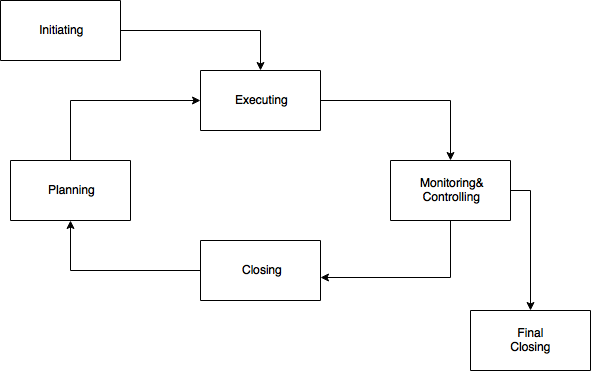
\includegraphics[scale=0.35]{Images/Implementation/Agile_Planning}
	\caption{Agile Planning Strategy}
\end{figure}
After this part, there will be a cycle of phases called respectively: Executing, monitoring\&Controlling, Closing and Planning. 
Every cycle round has as input a specific process to accomplish, that is divided between the various team’s parts. After executing all the tasks in a precise given timeframe, the work is checked by all the parts, customers included. When an agreemnt is reached, it will follow another planning phase that will contain also the corrections that will result after the agreement.
This cycle is repeated until the end of the project, when all the functionalities stated in the RASD will be covered.

\newpage
\mysubsection{Team structure}
Our team will be composed by two main parts :
\begin{itemize}
	\item \emph{Developers :} people devoted to implement the software.
	
	\item \emph{Testers :} people devoted to test the software functionalities.
	
	\item \emph{Front-End Team :} developers appointed to implement the system’s front end.
	
	
	\item \emph{Back-End Team :} developers appointed to implement the application logic of the system.
	
	\item \emph{Supervisors :} developers that belongs to the Back-End Team or to the Front-End Team and that have the main task of having any time the picture of all the their team work.
\end{itemize}

\mysubsection{Implementation and testing plan}
The work will be divided in sub-milestone from a minimum of one to a maximum of two weeks, and main-milestone every three or maximum four weeks. In these span of time all the teams have to complete the tasks that have been established in the previous planning phase. Every two days the different team's supervisors and a Tester’s team delegate will manage a meeting for speaking about their team progress and they will give directive for proceeding basically at the same speed. 
In the while, the Tester team will work on the \emph{white-box} units test for the functionalities that the developer’s teams are implementing.
When the sub-milestone’s day come, the Tester team will have from a minimum of a day to a maximum of 3 days for testing the functionalities and give the results to the development team that will have to fix the eventual bugs.

During the week before the the milestone’s day, the Tester team has to perform an \emph{integration test} of the components and give the result to the development teams that has to release a beta version to restrict and selected group of people for the milestone day. In this way, will be performed also an incremental \emph{User acceptance test} on the work that has been performed. Futrhemore, there will take place a meeting with the customer and their needs and doubts will be discuss and taken into account in the next planning phase.

The precice duration of the timeframe will be established step by step taking into account the minimum and maximum span on time given above and that the project has to be completed in maximum of 16 weeks.

\begin{figure}[H]
	\centering
	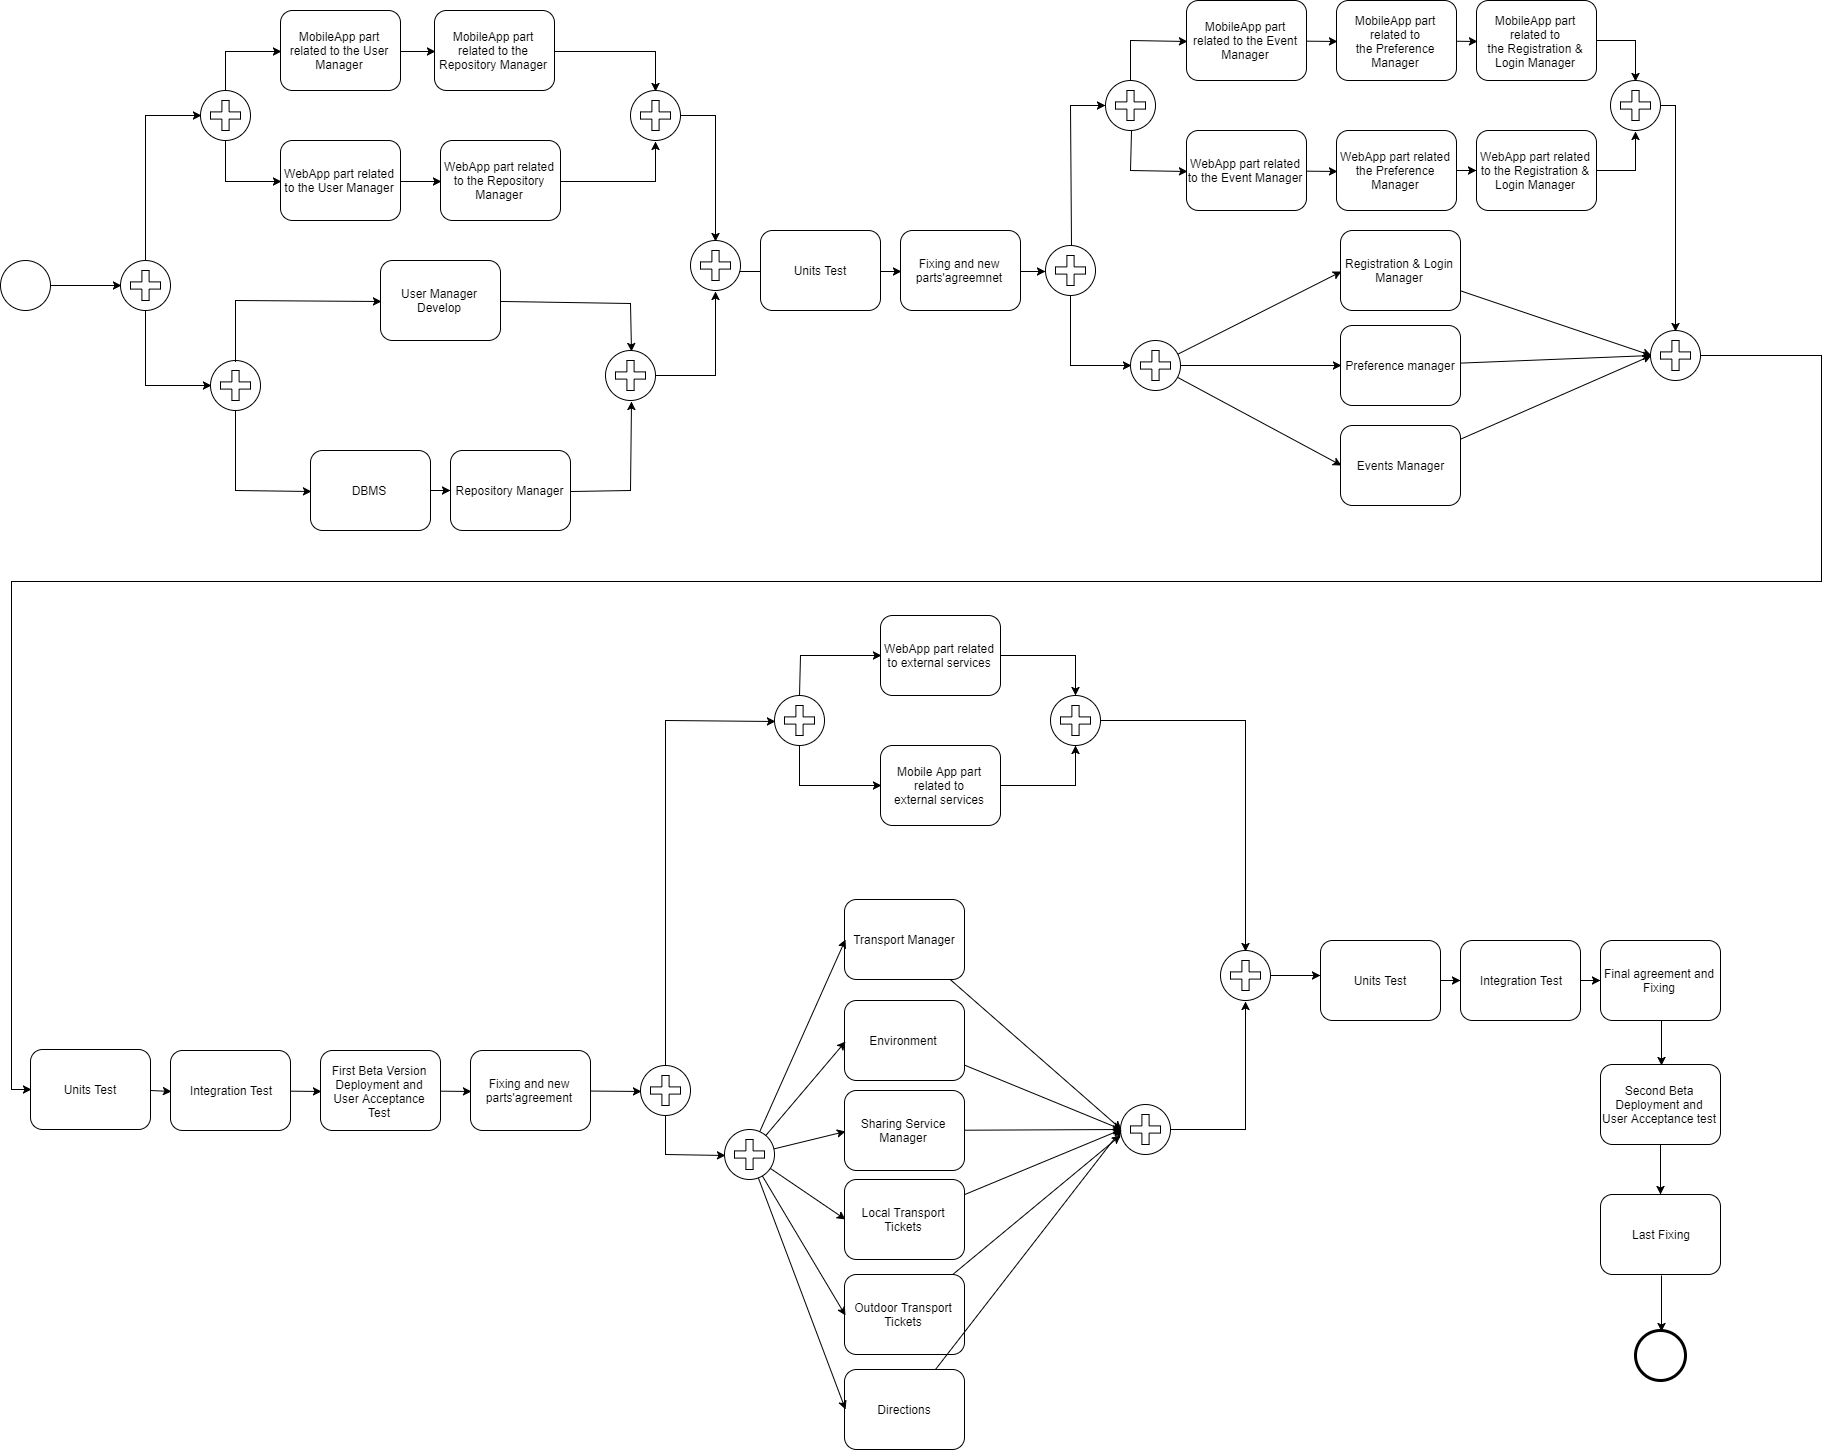
\includegraphics[scale=0.22]{Images/Implementation/Implementation_Flow}
	\caption{Implementation Flow}
\end{figure}

\mysubsection{Possible risks}
\begin{tabular}[H]{p{7cm}|c|c}
	Risk & Probability & Effects\\
	\hline
	\rule{0pt}{4ex} Budget Problems & Low & Catastrophic\\
	\hline
	\rule{0pt}{4ex} Time for Implementing a Function Exceed & Medium & Serious\\
	\hline
	\rule{0pt}{4ex} Team’s Members not Available in a Critic Moments & Medium & Catastrophic\\
	\hline
	\rule{0pt}{4ex} Impossibility to Recruit Staff with Required Skills & Medium & Serious
\end{tabular}

\mysubsection{Possible solutions}
\begin{itemize}
	\item \emph{Budget problems :}specify before starting all the functionalities and realize prevision of the costs and agree with the customers a margin of budget that could increase for unpredicted situation during the development.
	
	\item \emph{Time for implementing a function exceed :}agree with the stakeholder a span of time of delay that they can accept for unpredicted problems.
	
	\item \emph{Team’s member not available in critic moment :} being sure that at least one of the supervisors could substitute a team member in case of necessity
	
	\item \emph{Impossibility to recruit staff with required skills :} advices the customers about possible delete and be ready with a table of COTS to buy in case of needs with the correspondent costs.
	
\end{itemize}